\documentclass[a4paper,11pt]{amsart}
\usepackage{amsmath, amsthm, amsfonts, amssymb, amscd}
\usepackage{color}
\usepackage[ansinew]{inputenc}
\usepackage[colorlinks]{hyperref}
\usepackage{tikz}
\usetikzlibrary{decorations.markings}

\begin{document}

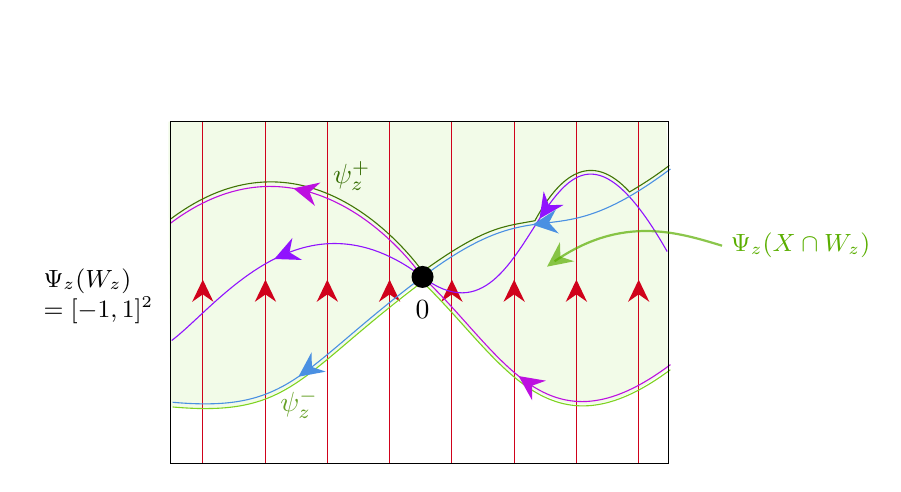
\begin{tikzpicture}[x=0.75pt,y=0.75pt,yscale=-1.5,xscale=1.5]

\draw [draw opacity=0][fill={rgb, 255:red, 126; green, 211; blue, 33 }  ,fill opacity=0.1 ]   (198.93,60.17) .. controls (199,108.79) and (199.6,125.79) .. (199.46,151.47) .. controls (235,156.59) and (244.2,139.79) .. (279.75,111.22) .. controls (303.2,133.39) and (322,169.79) .. (359.38,139.39) .. controls (359.12,108.26) and (359.6,88.19) .. (358.93,60.17) ;
\draw [color={rgb, 255:red, 208; green, 2; blue, 27 }  ,draw opacity=1 ]   (250,60) -- (250,170) ;
\draw [shift={(250,110.9)}, rotate = 90] [fill={rgb, 255:red, 208; green, 2; blue, 27 }  ,fill opacity=1 ][line width=0.08]  [draw opacity=0] (7.14,-3.43) -- (0,0) -- (7.14,3.43) -- (4.74,0) -- cycle    ;
\draw [color={rgb, 255:red, 208; green, 2; blue, 27 }  ,draw opacity=1 ]   (270,60) -- (270,170) ;
\draw [shift={(270,110.9)}, rotate = 90] [fill={rgb, 255:red, 208; green, 2; blue, 27 }  ,fill opacity=1 ][line width=0.08]  [draw opacity=0] (7.14,-3.43) -- (0,0) -- (7.14,3.43) -- (4.74,0) -- cycle    ;
\draw [color={rgb, 255:red, 208; green, 2; blue, 27 }  ,draw opacity=1 ]   (290,60) -- (290,170) ;
\draw [shift={(290,110.9)}, rotate = 90] [fill={rgb, 255:red, 208; green, 2; blue, 27 }  ,fill opacity=1 ][line width=0.08]  [draw opacity=0] (7.14,-3.43) -- (0,0) -- (7.14,3.43) -- (4.74,0) -- cycle    ;
\draw [color={rgb, 255:red, 208; green, 2; blue, 27 }  ,draw opacity=1 ]   (310,60) -- (310,170) ;
\draw [shift={(310,110.9)}, rotate = 90] [fill={rgb, 255:red, 208; green, 2; blue, 27 }  ,fill opacity=1 ][line width=0.08]  [draw opacity=0] (7.14,-3.43) -- (0,0) -- (7.14,3.43) -- (4.74,0) -- cycle    ;
\draw [color={rgb, 255:red, 208; green, 2; blue, 27 }  ,draw opacity=1 ]   (330,60) -- (330,170) ;
\draw [shift={(330,110.9)}, rotate = 90] [fill={rgb, 255:red, 208; green, 2; blue, 27 }  ,fill opacity=1 ][line width=0.08]  [draw opacity=0] (7.14,-3.43) -- (0,0) -- (7.14,3.43) -- (4.74,0) -- cycle    ;
\draw [color={rgb, 255:red, 208; green, 2; blue, 27 }  ,draw opacity=1 ]   (350,60) -- (350,170) ;
\draw [shift={(350,110.9)}, rotate = 90] [fill={rgb, 255:red, 208; green, 2; blue, 27 }  ,fill opacity=1 ][line width=0.08]  [draw opacity=0] (7.14,-3.43) -- (0,0) -- (7.14,3.43) -- (4.74,0) -- cycle    ;
\draw [color={rgb, 255:red, 208; green, 2; blue, 27 }  ,draw opacity=1 ]   (230.13,60) -- (230.13,170) ;
\draw [shift={(230.13,110.9)}, rotate = 90] [fill={rgb, 255:red, 208; green, 2; blue, 27 }  ,fill opacity=1 ][line width=0.08]  [draw opacity=0] (7.14,-3.43) -- (0,0) -- (7.14,3.43) -- (4.74,0) -- cycle    ;
\draw [color={rgb, 255:red, 208; green, 2; blue, 27 }  ,draw opacity=1 ]   (210,60) -- (210,170) ;
\draw [shift={(210,110.9)}, rotate = 90] [fill={rgb, 255:red, 208; green, 2; blue, 27 }  ,fill opacity=1 ][line width=0.08]  [draw opacity=0] (7.14,-3.43) -- (0,0) -- (7.14,3.43) -- (4.74,0) -- cycle    ;
\draw [color={rgb, 255:red, 126; green, 211; blue, 33 }  ,draw opacity=1 ]   (200.33,151.8) .. controls (238.61,155.23) and (240.62,141.54) .. (280.62,111.54) ;
\draw [color={rgb, 255:red, 126; green, 211; blue, 33 }  ,draw opacity=1 ]   (281.01,112.08) .. controls (306.6,137.08) and (321.1,168.99) .. (360.18,139.83) ;
\draw [color={rgb, 255:red, 65; green, 117; blue, 5 }  ,draw opacity=1 ]   (280.91,108.07) .. controls (300.86,93.7) and (306.91,93.81) .. (316.66,91.98) .. controls (324.46,77.7) and (334.41,68.98) .. (347.08,82.73) .. controls (352.16,79.72) and (355.48,77.51) .. (359.84,74.24) ;
\draw [color={rgb, 255:red, 144; green, 19; blue, 254 }  ,draw opacity=1 ]   (200.01,130.44) .. controls (214.7,119.42) and (241.99,80.77) .. (280.57,110.03) .. controls (319.15,139.3) and (318.3,30.15) .. (359.15,101.87) ;
\draw [shift={(232.96,104.27)}, rotate = 336.35] [fill={rgb, 255:red, 144; green, 19; blue, 254 }  ,fill opacity=1 ][line width=0.08]  [draw opacity=0] (8.04,-3.86) -- (0,0) -- (8.04,3.86) -- (5.34,0) -- cycle    ;
\draw [shift={(318.13,91.36)}, rotate = 304.37] [fill={rgb, 255:red, 144; green, 19; blue, 254 }  ,fill opacity=1 ][line width=0.08]  [draw opacity=0] (8.04,-3.86) -- (0,0) -- (8.04,3.86) -- (5.34,0) -- cycle    ;
\draw [color={rgb, 255:red, 65; green, 117; blue, 5 }  ,draw opacity=1 ]   (199.77,91.36) .. controls (239.77,61.36) and (271.69,96.33) .. (280.39,107.98) ;
\draw [color={rgb, 255:red, 74; green, 144; blue, 226 }  ,draw opacity=1 ]   (280.57,110.03) .. controls (320.57,80.03) and (320.2,105.35) .. (360.2,75.35) ;
\draw [shift={(315.89,93.26)}, rotate = 352.84] [fill={rgb, 255:red, 74; green, 144; blue, 226 }  ,fill opacity=1 ][line width=0.08]  [draw opacity=0] (8.04,-3.86) -- (0,0) -- (8.04,3.86) -- (5.34,0) -- cycle    ;
\draw [color={rgb, 255:red, 74; green, 144; blue, 226 }  ,draw opacity=1 ]   (200.29,150.29) .. controls (238.57,153.71) and (240.57,140.03) .. (280.57,110.03) ;
\draw [shift={(240.71,142.08)}, rotate = 323.91] [fill={rgb, 255:red, 74; green, 144; blue, 226 }  ,fill opacity=1 ][line width=0.08]  [draw opacity=0] (8.04,-3.86) -- (0,0) -- (8.04,3.86) -- (5.34,0) -- cycle    ;
\draw [color={rgb, 255:red, 189; green, 16; blue, 224 }  ,draw opacity=1 ]   (280.57,110.03) .. controls (306.77,134.78) and (320.2,168.2) .. (360.2,138.2) ;
\draw [shift={(311.43,141.87)}, rotate = 35.27] [fill={rgb, 255:red, 189; green, 16; blue, 224 }  ,fill opacity=1 ][line width=0.08]  [draw opacity=0] (8.04,-3.86) -- (0,0) -- (8.04,3.86) -- (5.34,0) -- cycle    ;
\draw [color={rgb, 255:red, 189; green, 16; blue, 224 }  ,draw opacity=1 ]   (199.63,92.78) .. controls (239.63,62.78) and (271.91,97.92) .. (280.57,110.03) ;
\draw [shift={(239.09,81.59)}, rotate = 13.44] [fill={rgb, 255:red, 189; green, 16; blue, 224 }  ,fill opacity=1 ][line width=0.08]  [draw opacity=0] (8.04,-3.86) -- (0,0) -- (8.04,3.86) -- (5.34,0) -- cycle    ;
\draw   (199.71,60) -- (359.71,60) -- (359.71,170) -- (199.71,170) -- cycle ;
\draw  [draw opacity=0][fill={rgb, 255:red, 0; green, 0; blue, 0 }  ,fill opacity=1 ] (277.03,110.03) .. controls (277.03,108.08) and (278.62,106.49) .. (280.57,106.49) .. controls (282.53,106.49) and (284.11,108.08) .. (284.11,110.03) .. controls (284.11,111.99) and (282.53,113.57) .. (280.57,113.57) .. controls (278.62,113.57) and (277.03,111.99) .. (277.03,110.03) -- cycle ;
\draw [color={rgb, 255:red, 90; green, 174; blue, 0 }  ,draw opacity=0.7 ][line width=0.8]   (376.78,100) .. controls (362.89,95.82) and (344.89,89.94) .. (322.98,105.01) ;
\draw [shift={(320.58,106.73)}, rotate = 323.21] [fill={rgb, 255:red, 90; green, 174; blue, 0 }  ,fill opacity=0.7 ][line width=0.08]  [draw opacity=0] (8.04,-3.86) -- (0,0) -- (8.04,3.86) -- (5.34,0) -- cycle    ;

% Text Node
\draw (280.57,116.97) node [anchor=north] [inner sep=0.75pt]    {$0$};
% Text Node
\draw (241,145.33) node [anchor=north] [inner sep=0.75pt]  [color={rgb, 255:red, 101; green, 160; blue, 37 }  ,opacity=1 ]  {$\psi _{z}^{-}$};
% Text Node
\draw (251,83) node [anchor=south west] [inner sep=0.75pt]  [color={rgb, 255:red, 55; green, 110; blue, 5 }  ,opacity=1 ]  {$\psi _{z}^{+}$};
% Text Node
\draw (199.37,116.25) node [anchor=east] [inner sep=0.75pt]  [font=\small]  {$ \begin{array}{l}
\Psi _{z}( W_{z})\\
=[ -1,1]^{2}
\end{array}$};
% Text Node
\draw (378.78,100) node [anchor=west] [inner sep=0.75pt]  [font=\small,color={rgb, 255:red, 90; green, 174; blue, 0 }  ,opacity=1 ]  {$\Psi _{z}( X\cap W_{z})$};


\end{tikzpicture}

\end{document}